\section{MCU}

\subsection{External Bus Interface}
\begin{wrapfigure}[14]{r}{6cm}
    \centering
    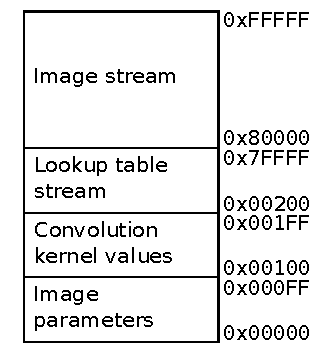
\includegraphics[]{img/EbiAddressSpace.pdf}
    \caption{EBI Address Space}
    \label{fig:EbiAddressSpace}
\end{wrapfigure}
The FPGA and the MCU is connected through an EBI bus.
This interface is supported natively by the MCU and can therefore be handled by its built-in direct memory access (DMA) unit, which hopefully makes streaming video from the MCU faster, more reliable and easier to implement.

In addition to streaming video, the MCU should also control the operation of Daisy.
To accomplish this, we utilize the large address space available.
An overview can be seen in figure \ref{fig:EbiAddressSpace}.

\subsubsection{Daisy Configuration}
Configuration values for Daisy have their own memory addresses so that configuring daisy is only a matter of saving the correct values to the correct addresses.

Note that the amount of space allocated to each group of options in figure \ref{fig:EbiAddressSpace} is more than needed.
This simplifies the process of adding more configuration options if required at a later point.

\subsubsection{Streaming Data}
Some data is of unknown or unlimited length. This data is streamed to daisy by reusing the same addresses several times.
By assigning a large block of the memory space to each data stream, we can utilize the DMA without having to worry about unintendedly overwriting configuration values.

The reuse of addresses also provides a natural sync point for the video stream;
each write to the first address of the address space reserved for streaming video is assumed to be a \textit{frame sync}.
That is, it signals the start of a new frame.
This makes the system less fragile as Daisy can catch up with the data stream should it ever end up being out of sync.
